\label{capitolo6}
\section{Test di circuiti digitali}
I test si collocano dopo la progettazione e dopo la fabbricazione. Questo implica dei problemi di competenza tra pogettisti e fabbricanti. infatti � necessario che tutto ci� che esce dalla progettazione sia oltre che verificato anche testato.\\
Il principio del testing � introdurre un vettore di input in ingresso al circuito e confrontare l'output con la versione corretta.
I test devono coprire il maggior numero di guasti possibili ma non devono essere troppo lunghi.\\
Il modo migliore � analizzare prima i possibili guasti:
\begin{itemize}
\item Individuando i possibili difetti nel processo di produzione
\item Sviluppando simulatori di guasto
\item Sviluppando generatori di test
\item Trovare metodi di quantificazione dell'efficenza dei test.
\end{itemize}Esiste una distinzione tra \emph{verifica} e \emph{test} con il primo termine si intende un meccanismo di analisi che si assicura che il progetto di sintesi assicuri il corretto funzionamento del sistema. Il processo di test, invece, assicura che il sistema fisico non ha difetti.\\
Esistono diversi livelli a cui fare il testing. Il livello pi� basso � quello di chip poi di board ed infine a livello di sistema; il costo di test cresce di un fattore 10 man mano che saliamo di livello nel test.
\subsection{Fault Modeling}
Solitamente i vettore di I/O che si utilizzano nella verifica sono inadeguati per scovare i difetti nella fabricazione in quanto essi sono spesso troppo numerosi e non sempre analizzabili. In questo caso ci viene in soccorso il \emph{fault model} che identifica i punti da testare ed � effettivamente misurabile la quantit� di guasti che si testano.\\
Per progettare un buon modello di test bisogna conoscere i guasti pi� comuni che si possono presentare che sono:
\begin{itemize}
\item apertura o cortocircuito di transitor
\item guasti alla memoria
\item guasti funzionali
\item errori da ritardo
\item errori analogici
\item stuck-at
\end{itemize}
\subsubsection{Guasto stuck-at}
I guasto di tipo stuck-at si ha quando una singola linea \emph{(single stuck-at fault)} mantiene permanentemente il valore 0 o 1 e questo errore comporta un errore in uscita.\\
L'errore di singolo stuck-at � utile per individuare altri tipi di guasti ed inoltre � molto semplice da utilizzare.
Il numero di siti di guasto � dato da:
$n\_ingressi\_primari+n\_porte+n\_bracci\_fanout$
Due guasti $f_1$ e $f_2$ si dicono equivalenti se tutti i test che individuano $f_1$ individuano anche $f_2$. Ogni singolo guasto di un circuito logico pu� essere suddiviso in un sottoinsieme disgiunto nel quale i guasti sono tra loro equivalenti.
\paragraph{Dominanza di guasti}
Se tutti i testi di un qualsiasi guasto $f_1$ individuano un ulteriore guasto $f_2$ allora si dice che $f_2$ domina $f_1$ e si pu� togliere dalla lista dei guasti.
\paragraph{Checkpoints}
Tutti gli ingressi primari e i rami dei fanout vengono chiamati checkpoints. Esiste un teorema che afferma che un test che controlla tutti i guasti su tutti i checkpoints individua tuttti i guasti del circuito.
\subsection{Fault simulation}
Dato un circuito un insieme di vettori di ingresso e un modello di guasto calcolato con i metodi precedenti ci si pone il problema di determinare quale sar� la copertura di guasti testati dall'insieme di vettori di test dati.
Lo scopo principale di questa simulazione � quello di valutare la bont� dei test effettuati e di individuare quelle zone non coperte dai test selezionati.\\
Lo scenario in cui la \emph{fault simulation} si va a collocare � un ambiente in cui abbiamo un circuito logico con diversi livelli di segnale o un sistema ad alto livello nel quale si possono verificare guasti sui singoli pin dei componenti; inoltre i sistemi potranno avere due o tre livelli di segnale per quanto riguarda i circuiti puramente logici o fino a quattro livelli di segnale per i circuiti sequenziali con C-MOS. Infine potremmo avere circuiti ideali con tempi di ritardo nulli per circuiti combinatori e sequenziali o con ritardi negli altri casi.\\
I guasti che andremo ad analizzare saranno di tipo single stuck-at e ove possibile per guasti equivalenti si andr� ad analizzare solo il guasto collassato.\\
\subsubsection{Simulazione seriale}
L'algoritmo consiste nell'ingnettare un singolo guasto in uno dei punti del circuito e di simulare il circuito con guasto con tutti i vettori di ingresso a disposizione e comparando il risultato con quelli salvati. Se la risposta differisce dal risultato previsto si sospende la simulazione e si comunica l'individuazione del guasto.
I vantaggi di questo algoritmo sono la facile implementazione e la grande variet� di quasti che possono essere simulati.\\
Gli svantaggi per� sono che siamo costretti a modificare la netlist del circuito ad ogni simulazione. Esistono per� degli accorgimenti che rendono il sistema meno costoso. Il primo � la verifica se una rete � \emph{fault} o \emph{fault-free} in questo caso si pu� impostare il valore in uscita dalla sottorete al valore errato o corretto a seconda dei casi. Il secondo metodo detto \emph{Mux} prevede di calcolare il valore finale utilizzando oltre all segnale anche il valore di una variabile ausiliaria.
Questo tipo di simulazione per� resta comunque inefficace in quanto richiede simulazioni ripetute e tempi di CPU proibitivi.
\subsubsection{Simulazione parallela}
Si tratta di una tecnica a codice compilato ottima per circuiti con due stati (0,1) sfrutta il parallelismo delle operazioni logiche nei bit delle parole di memoria. Ogni passo della simulazione � in grado di simulare fino a $w-1$ guasti del circuito dove $w$ � la lunghezza della parola; tuttavia questo meccanismo non � sfruttabile per circuiti non booleani o con tempi critici di ritardo.
\begin{figure}[thb]
\centering
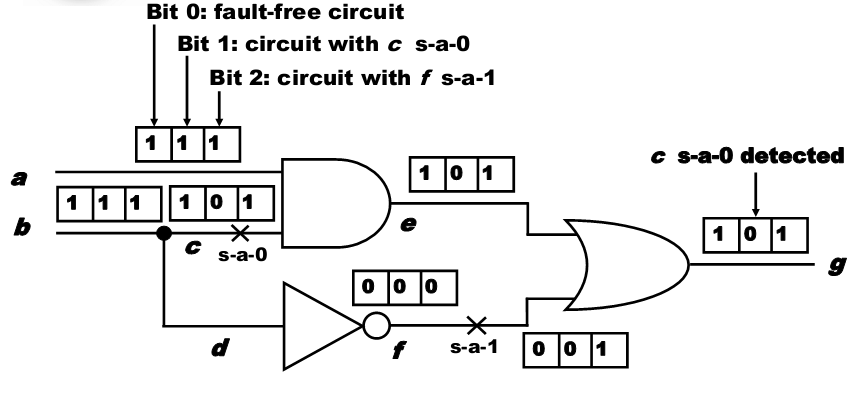
\includegraphics[width=12cm]{img/simul_paral.png}
\caption{Esempio di simulazione parallela}
\end{figure}
\subsubsection{Simulazione di guasto deduttiva}
Questo tipo di simulazione � una simulazione ad un passo; ogni linea k contiene una lista dei possibili guasti che si possono verificare su k. Seguendo i valori della simulazione i valori in uscita dalle porte vengono aggiornati secondo regole teoriche e la lista dei guasti. Il problema della simulazione � che non pu� essere utilizzata su circuiti non booleani a causa delle regole teoriche e i ritardi non vengono ben espressi.
\subsubsection{Simulazione di guasto concorrente}
Una simulazione basata su eventi nel quale si simula il circuito privo di errori e solo quelle parti in cui il guasto causa una differenza di segnale.
Ogni gate contiene una lista di tutte le possibili configurazioni di guasto di quel gate. Ogni possibile configurazione viene simulata. Questo fa si che la simulazione sia molto veloce ma consumi una grande quantit� di memoria.
